% MSV Evolution -- IEEE conference paper (2-page target)
% Overleaf: create a Blank Project, delete its main.tex, upload this file as main.tex,
% and compile with pdfLaTeX. Self-contained -- no external images, no .bib file needed.
%
% Source basis: docs/MSV_EVOLUTION_IEEE_PAPER_DRAFT.md (prose), reconciled against
% docs/MSV_BUILD_MILESTONE_FACT_CHECK.md (approved numbers) and, for the electrode
% topology of the two field units, directly against
% arduino/MSV2_Moisture_BLE_Sleep_Alocasia/MSV2_Moisture_BLE_Sleep_Alocasia.ino and
% arduino/MSV2_Moisture_BLE_Sleep/MSV2_Moisture_BLE_Sleep.ino (see the correction note
% at \S II.B: the fact-check doc and both outline/draft docs had Alocasia's topology and
% pulldown value backwards -- 56 kOhm dual-plate -- the firmware source says 100 kOhm
% single-plate). Author: verify every remaining figure against live hardware / the
% receiver's /device endpoint before submission -- see the checklist at the end of this
% file (kept as a LaTeX comment so it does not render).

\documentclass[conference]{IEEEtran}
\usepackage{amsmath}
\usepackage{amssymb}
\usepackage{textcomp}
\usepackage{graphicx}
\usepackage{tikz}
\usetikzlibrary{arrows.meta, positioning, calc}
\usepackage{booktabs}
\usepackage{url}

\begin{document}

\title{Evolution of the MSV Soil-Moisture Platform: From 555-Timer Sensing to a Switched Lock-In Probe}

\author{
\IEEEauthorblockN{Sam Amezcua}
\IEEEauthorblockA{Department of Electrical and Computer Engineering\\
University of California, Davis\\
Davis, California, USA\\
scamezcua@ucdavis.edu}
}

\maketitle

\begin{abstract}
This paper summarizes four generations of a capacitive soil-moisture sensor. MSV1 used cascaded
555 timers but compressed the useful response because its analog stage was designed for
80--220\,pF while measurements reached 274\,pF--1.28\,nF. MSV2 replaced analog conversion with
digitally timed relaxation oscillation and added Bluetooth Low Energy (BLE), an ESP32-S3 receiver,
cloud history, and plant-specific calibration. Field use exposed clock quantization, supply
coupling, electrode-bias risk, flash leakage, and receiver/cloud defects. MSV3 is a work in
progress using an FDC2214 resonant converter, a TMUX1109 to route two electrodes through four
states, and solar harvesting. Bring-up verified a 17-byte packet, 900 consecutive post-repair
samples, and 10--15\,\textmu A timed-sleep current. Wet-soil stability and energy-neutral operation
remain open. A prefabrication MSV4 design replaces the shallow interdigitated electrode with a
wide-spaced, polarity-reversing probe and synchronous lock-in readout. A two-dimensional complex
electrostatic model predicts approximately fivefold greater median sensing depth and half the
lossless interface-gap sensitivity, while also identifying soil conductivity and physical contact
as the dominant remaining confounds. These MSV4 results are numerical predictions, not field data.
\end{abstract}

\begin{IEEEkeywords}
capacitive soil-moisture sensing, Bluetooth Low Energy, FDC2214, lock-in detection, numerical
electrostatics, nRF52840, energy harvesting, wireless sensor node
\end{IEEEkeywords}

\section{Introduction}
Capacitive electrodes reduce the corrosion and polarization risk of low-cost resistive soil
probes. The MSV project progressed from an analog proof of concept (MSV1), through a connected
nRF52840/ESP32-S3 platform (MSV2), to a dedicated capacitance-converter and solar-assisted probe
(MSV3), and finally to a prefabrication switched lock-in sensor with wider electrode spacing
(MSV4). The objective remained a repeatable, low-power moisture indicator with wireless history.
This paper emphasizes the measured shortcomings that motivated each transition and clearly
separates measured results from MSV4 simulation predictions.

\section{Architecture Evolution}

\subsection{MSV1: Analog Frequency-to-Voltage Measurement}
MSV1 used an interdigitated PCB comb, astable and monostable 555 timers, an RC low-pass filter,
and a comparator/LED alarm \cite{amezcua2026msv1}. Potting-soil frequency changed from
approximately 27\,kHz dry to 7.5\,kHz wet, while extracted capacitance ranged from 274\,pF dry to
approximately 1.28\,nF saturated. The downstream voltage nonetheless remained near
1.07--1.10\,V because the RC chain was sized for a much smaller predicted range
(80--220\,pF). A 100\,k$\Omega$ feedback resistor caused comparator latching; removing it
produced near-threshold flicker instead. Direct digital timing in MSV2 preserved the useful
frequency response without this analog compression.

\subsection{MSV2: Connected Digital Relaxation Oscillator}
The Seeed XIAO nRF52840 Sense probe counts repeated capacitive charge/discharge transitions,
applies burst/median filtering, and broadcasts raw values in non-connectable BLE advertisements
\cite{project_oscillator_report}. Early MSV2 sensing fixed the drive direction against a grounded
return; a later dual-plate rework alternates which electrode drives and which senses each cycle to
reduce sustained DC bias.

\textbf{Correction to earlier project notes:} the two current field units are \emph{not} the same
topology. Only the Thaumatophyllum unit has been migrated to the dual-plate rework (10\,k$\Omega$
pulldown per plate); the Alocasia unit still runs the original single-plate firmware against a
grounded return, with a 100\,k$\Omega$ pulldown. This is stated directly in that probe's own
firmware source and is the opposite of what an earlier internal fact-check pass concluded (it had
recorded Alocasia as 56\,k$\Omega$ dual-plate, a value that does not appear in any firmware or
hardware source in the repository). The two units therefore differ in topology as well as raw
range and must not be presented as two instances of one dual-plate design differing only by
resistor value.

An ESP32-S3 receiver performs calibration, display, history recovery, and cloud upload; a
progressive web application presents the stored data. The probe uses timed System-ON sleep,
approximately 10\,s wake/check intervals, and approximately 60\,s advertisements.

\subsection{MSV3: Resonant Conversion, Electrode Multiplexing, and Solar Power}
MSV3 replaces GPIO timing with an FDC2214 28-bit capacitance-to-digital converter and a
6.8\,\textmu H / 270\,pF LC tank \cite{ti_fdc2214}. A TMUX1109 routes two electrodes through four
states: two swapped capacitance-measurement phases and two auxiliary EC-check/bare-tank reference
phases \cite{ti_tmux1109} -- a two-electrode, four-state design, not an arbitrary $N$-channel
array. The E73-2G4M08S1C nRF52840 module has no 32.768\,kHz crystal, requiring firmware to select
the internal low-frequency RC oscillator before the SoftDevice/FreeRTOS start
\cite{nordic_nrf52840, project_lfclk_hang}; this is enforced by a build script rather than left to
manual discipline. The power path combines a BQ25504 energy-harvesting front end, a BQ25170
charger, and a TPS7A0233 3.3\,V regulator \cite{ti_bq25504}. MSV3 preserves the MSV2 receiver and
cloud path unchanged; its observed live packet is 17 bytes. A 23-byte die-temperature/bare-tank
reference format is compile- and cloud-tested but not confirmed flashed to a field unit.

\subsection{MSV4: Wide-Spaced Electrodes and Synchronous Detection}
MSV4 retains the E73 nRF52840 and solar power architecture but replaces the resonant FDC2214 path
with two FSUSB42 dual analog switches. One switch alternately drives electrode A or B through
1\,k$\Omega$ while grounding the other; the second synchronously chops both the sensed voltage and
a pre-resistor drive-reference voltage into matched 100\,k$\Omega$/1\,nF averaging filters. TIMER3,
GPIOTE, and PPI generate phase-stable 1--4\,MHz excitation and four-phase sampling without
software-timed edges. The drive-reference channel permits complex-ratio calibration of GPIO
amplitude and common switch timing, while a thermistor at the blade tip supports first-order
temperature correction. The fabricated hardware and its soil calibration remain future work.

Fig.~\ref{fig:arch} summarizes the four signal paths and the receiver/cloud stage shared by MSV2
through MSV4.

\begin{figure*}[!t]
\centering
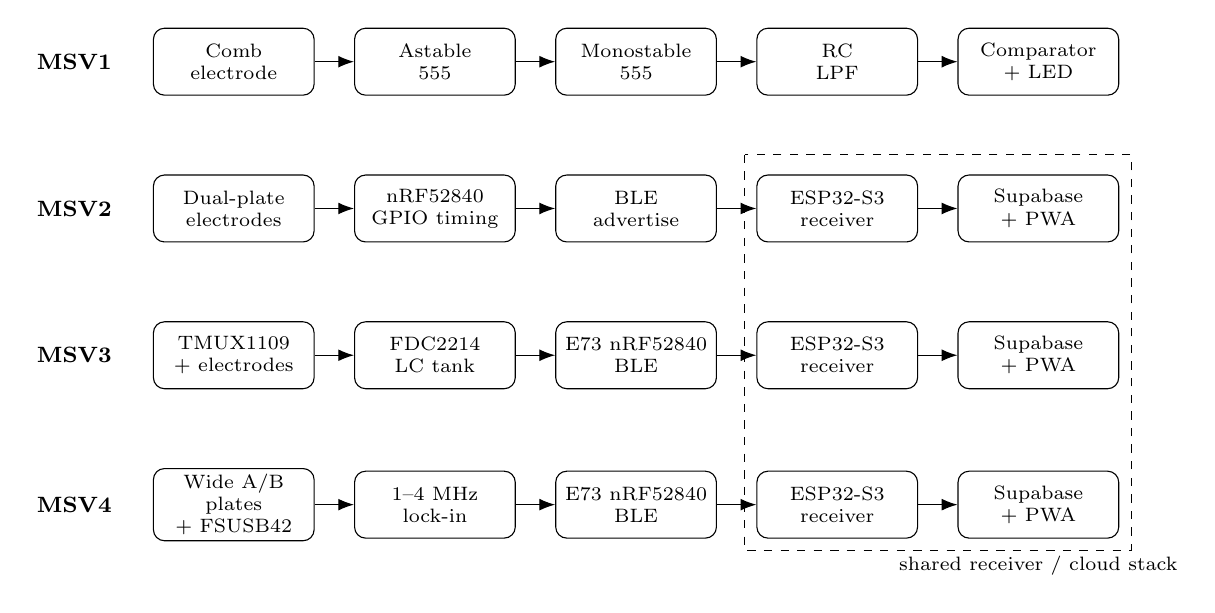
\begin{tikzpicture}[
  box/.style={draw, rounded corners, align=center, font=\scriptsize, text width=1.9cm,
              minimum height=0.85cm, inner sep=2pt},
  arr/.style={-{Latex[length=2mm]}},
  node distance=5mm
]
  % MSV1 row
  \node[box] (m1a) {Comb\\electrode};
  \node[box, right=of m1a] (m1b) {Astable\\555};
  \node[box, right=of m1b] (m1c) {Monostable\\555};
  \node[box, right=of m1c] (m1d) {RC\\LPF};
  \node[box, right=of m1d] (m1e) {Comparator\\+ LED};
  \draw[arr] (m1a) -- (m1b);
  \draw[arr] (m1b) -- (m1c);
  \draw[arr] (m1c) -- (m1d);
  \draw[arr] (m1d) -- (m1e);
  \node[font=\footnotesize\bfseries, left=4mm of m1a, anchor=east] {MSV1};

  % MSV2 row
  \node[box, below=10mm of m1a] (m2a) {Dual-plate\\electrodes};
  \node[box, right=of m2a] (m2b) {nRF52840\\GPIO timing};
  \node[box, right=of m2b] (m2c) {BLE\\advertise};
  \node[box, right=of m2c] (m2d) {ESP32-S3\\receiver};
  \node[box, right=of m2d] (m2e) {Supabase\\+ PWA};
  \draw[arr] (m2a) -- (m2b);
  \draw[arr] (m2b) -- (m2c);
  \draw[arr] (m2c) -- (m2d);
  \draw[arr] (m2d) -- (m2e);
  \node[font=\footnotesize\bfseries, left=4mm of m2a, anchor=east] {MSV2};

  % MSV3 row
  \node[box, below=10mm of m2a] (m3a) {TMUX1109\\+ electrodes};
  \node[box, right=of m3a] (m3b) {FDC2214\\LC tank};
  \node[box, right=of m3b] (m3c) {E73 nRF52840\\BLE};
  \node[box, right=of m3c] (m3d) {ESP32-S3\\receiver};
  \node[box, right=of m3d] (m3e) {Supabase\\+ PWA};
  \draw[arr] (m3a) -- (m3b);
  \draw[arr] (m3b) -- (m3c);
  \draw[arr] (m3c) -- (m3d);
  \draw[arr] (m3d) -- (m3e);
  \node[font=\footnotesize\bfseries, left=4mm of m3a, anchor=east] {MSV3};

  % MSV4 row
  \node[box, below=10mm of m3a] (m4a) {Wide A/B plates\\+ FSUSB42};
  \node[box, right=of m4a] (m4b) {1--4 MHz\\lock-in};
  \node[box, right=of m4b] (m4c) {E73 nRF52840\\BLE};
  \node[box, right=of m4c] (m4d) {ESP32-S3\\receiver};
  \node[box, right=of m4d] (m4e) {Supabase\\+ PWA};
  \draw[arr] (m4a) -- (m4b);
  \draw[arr] (m4b) -- (m4c);
  \draw[arr] (m4c) -- (m4d);
  \draw[arr] (m4d) -- (m4e);
  \node[font=\footnotesize\bfseries, left=4mm of m4a, anchor=east] {MSV4};

  % shared receiver/cloud annotation
  \draw[dashed] ($(m2d.north west)+(-0.15,0.25)$) rectangle ($(m4e.south east)+(0.15,-0.15)$);
  \node[font=\scriptsize, below=1mm of m4e, anchor=north] {shared receiver / cloud stack};
\end{tikzpicture}
\caption{Four-generation signal path. MSV1 converts frequency to a threshold voltage entirely in
analog hardware. MSV2--MSV4 measure digitally at the probe and share the same ESP32-S3 receiver
and cloud stack; the sensing front end evolves between generations.}
\label{fig:arch}
\end{figure*}

\section{Tests, Milestones, and Corrective Work}
The main verified events are summarized in Table~\ref{tab:milestones}. Dates indicate the day
documented in the repository; they do not imply second-level deployment accuracy.

\begin{table}[!t]
\caption{Selected Verified Project Events}
\label{tab:milestones}
\centering
\footnotesize
\begin{tabular}{@{}p{0.16\linewidth}p{0.32\linewidth}p{0.42\linewidth}@{}}
\toprule
\textbf{Date (2026)} & \textbf{Test / milestone} & \textbf{Result / significance} \\
\midrule
Jul.\ 24 & BLE loss test & 198/200 advertisements received in 10\,min; 1.00\% observed loss. \\
Jul.\ 24--25 & In-soil RC and oscillator tests & One-shot RC timing was impractical; free-running
relaxation frequency became the MSV2 method. \\
Jul.\ 31 & RTC timing analysis & A 1\,ms gate produced quantized plateaus; a 5\,ms window reduced
the artifact. \\
Aug.\ 9 & Probe power investigation & QSPI flash left active at $\sim$1.3--1.5\,mA; deep-power-down
fix restored expected life on both probes. \\
Aug.\ 12--14 & Receiver/UI stabilization & Touch/SPI, animation, BLE/cloud coexistence, caching,
and other defects corrected. \\
Aug.\ 21 & MSV3 LFCLK and sleep-current repair & LFRC-at-startup eliminated a 115--122-sample
freeze (900 consecutive samples after) \cite{project_lfclk_hang}. Sleep current fell from
65--71\,\textmu A to 10--15\,\textmu A. \\
Aug.\ 22 & MSV3 production rollout & First MSV3 production probe/receiver observed live; 17-byte
high-resolution packet, lossless history batching, and full adaptive calibration documented
\cite{project_production_firmware}. \\
Aug.\ 23--25 & History recovery / filtering / pagination & Live/history consistency, centered
filtering, and an infinite-reload pagination defect corrected in successive receiver builds. \\
\bottomrule
\end{tabular}
\end{table}

MSV2's short measurement gate was quantized by the RTC tick, and supply voltage also shifted the
oscillator. More critically, QSPI flash remained awake at roughly 1.3--1.5\,mA and exhausted
150\,mAh batteries in four to six days. Receiver testing found BLE/TLS contention, touch/SPI
corruption, stale cached assets, and long-range history pagination defects
\cite{project_status_handoff}. These are system-integration failures rather than sensing-only
failures.

MSV3 initially froze after 115--122 samples because a post-startup low-frequency-clock
reconfiguration corrupted RTC1; selecting the internal RC oscillator at the board-variant level
(before FreeRTOS/SoftDevice start) produced 900 consecutive samples across two runs
\cite{project_lfclk_hang}. Disconnecting the battery-divider and charger-status pins before sleep
reduced timed-sleep current from 65--71\,\textmu A to 10--15\,\textmu A. Direct sunlight produced
6\,V open-circuit and 30\,mA short-circuit; roughly 10\,mA of battery charging was inferred from
voltage-rise behavior, not directly measured with an ammeter.

\section{MSV4 Electrode Field Simulation}
The prefabrication electrode was evaluated with a numerical rather than physical test apparatus.
The exact MSV4 cross-section was taken from the Sept.~18 IPC-2581 export: two 4.725\,mm plates
separated by 4.725\,mm, a grounded edge guard, an 81.1\,mm active length, 1.6\,mm FR4
($\epsilon_r=4.4$), and 20\,\textmu m solder mask ($\epsilon_r=3.8$). A two-dimensional
finite-volume model solved
\begin{equation}
 \nabla\!\cdot\!\left(\epsilon^*\nabla V\right)=0, \qquad
 \epsilon^*=\epsilon_0\epsilon_r-j\frac{\sigma}{\omega},
\end{equation}
with electrode A at 1\,V and electrode B plus the guard at 0\,V. Complex admittance per unit length
was obtained from the field-energy identity and multiplied by the active length. The fine mesh was
50\,\textmu m laterally and 10\,\textmu m through the mask; expanding the exterior domain from
20 to 45\,mm changed the $\epsilon_r=20$ result by less than 0.7\%. For a like-for-like geometry
comparison, an idealized MSV3-style 0.5\,mm-finger/1.0\,mm-gap pattern was assigned the same blade
width and extrusion length. Thus, Table~\ref{tab:fieldsolve} compares normalized geometries; its
MSV3 capacitances are not the complete in-circuit FDC2214 tank capacitance.

Penetration was calculated by replacing soil beyond depth $d$ with air and dividing the resulting
capacitance change by the full $\epsilon_r=20$ soil-to-air change. Interface sensitivity was found
by inserting a 10\,\textmu m air layer between solder mask and soil. These procedures produced the
results in Table~\ref{tab:fieldsolve}; the median sampled depth increases from approximately
0.2 to 1.0\,mm, while lossless air-gap sensitivity is halved. The absolute MSV4 capacitance is lower,
but the sensing volume is substantially less concentrated at the board surface, consistent with
the electrode-spacing dependence of fringing fields \cite{mamishev2004}.

\begin{table}[!t]
\caption{Modeled Electrode Comparison (Not Bench Data)}
\label{tab:fieldsolve}
\centering
\footnotesize
\begin{tabular}{@{}p{0.58\columnwidth}rr@{}}
\toprule
\textbf{Metric} & \textbf{MSV3-style} & \textbf{MSV4} \\
\midrule
Spatial period (mm) & 3.0 & 18.9 \\
Capacitance in air (pF) & 34.9 & 6.1 \\
Capacitance, lossless $\epsilon_r=20$ soil (pF) & 130.8 & 40.4 \\
Median signal depth (mm) & $\sim$0.2 & $\sim$1.0 \\
Signal within first 0.25\,mm (\%) & 55 & 19 \\
Signal within first 0.5\,mm (\%) & 80 & 32 \\
Signal within first 1.0\,mm (\%) & 95 & 50 \\
Signal within first 2.0\,mm (\%) & 98 & 70 \\
10\,\textmu m gap, lossless soil (\%) & $-17.0$ & $-8.5$ \\
10\,\textmu m gap, moist soil at 1\,MHz (\%) & $-58.5$ & $-42.5$ \\
\bottomrule
\end{tabular}
\end{table}

Conductive soil remains the dominant limitation. For the illustrative moist-soil case
($\epsilon_r=15$, $\sigma=0.02$\,S/m), the loss ratio $\sigma/(\omega\epsilon)$ falls from 24 at
1\,MHz to 6 at 4\,MHz, and the modeled 10\,\textmu m-gap error falls from 42.5\% to 24.8\%.
A 75\,\textmu m, $\epsilon_r=3$ coating reduces those errors to 21.1\% and 12.5\%, respectively.
Higher-frequency soil sensors likewise show reduced salinity and texture sensitivity
\cite{kizito2008}. Using explicit dry ($\epsilon_r=4$, $\sigma=0.002$\,S/m) and saturated
($\epsilon_r=25$, $\sigma=0.1$\,S/m) endpoints, the model gives $|Z|=2.31$\,k$\Omega$ and
227\,$\Omega$, respectively; this range supports the selected 1\,k$\Omega$ series resistor. The
4\,MHz firmware path compiles but has not yet been verified on hardware.

\section{Limitations and Next Work}
MSV3 still requires wet-soil calibration, FDC2214 drive-current/ring-down tuning, multi-day drift
measurement, and overcast/low-battery solar-recovery tests -- the latter is in progress as of this
writing on a probe that was fully discharged and released to run on solar power alone. Graded
conductivity sensing is not operational: the divider node is routed to P0.00, which has no ADC
capability on this MCU, so a bodge to an analog-capable pin plus a PCB revision are required. Die
temperature is MCU/electronics temperature and must not be labeled soil temperature. The current
receiver build should also be verified through its \texttt{/device} endpoint before presenting
results; checked-in source alone does not prove what is flashed to the physical unit.

MSV4 conclusions are presently limited to a two-dimensional, uniform-along-length,
electroquasistatic model with assumed material properties. End fringing, coating thickness and
water uptake, soil heterogeneity, packing gaps, frequency dispersion, switch/GPIO timing, and the
square-wave excitation harmonics require bench validation. The first experiment should compare
otherwise identical mask-only and approximately 75\,\textmu m-coated boards in controlled soil at
1, 2, and 4\,MHz while recording gravimetric water content, bulk conductivity, and the blade-tip
thermistor. The lock-in in-phase and quadrature terms must be calibrated as two empirical features;
they must not be labeled pure conductance and permittivity before that calibration.

\section{Conclusion}
MSV evolved from an analog proof of concept to a connected field platform, a dedicated resonant
converter, and a prefabrication switched lock-in probe. Its central lesson is that electrode
physics, clocking, power state, packet compatibility, receiver recovery, calibration, and history
handling must be validated together -- most of MSV2's hardest bugs were system-integration
failures, not sensing-principle failures. The MSV4 field model supports fabrication of the drawn
wide-spaced geometry, predicting approximately fivefold greater median sensing depth and half the
lossless interface-gap sensitivity of the normalized MSV3-style reference. Those predictions and
the proposed 4\,MHz operating point remain to be confirmed by controlled soil measurements.

\begin{thebibliography}{11}

\bibitem{amezcua2026msv1}
S. Amezcua, ``Design and Experimental Characterization of a Capacitive Soil Moisture Sensor Using a
555 Timer Architecture,'' EEC 284 final paper, Dept. Elect. Comput. Eng., Univ. California, Davis,
CA, USA, 2026.

\bibitem{ti_fdc2214}
Texas Instruments, ``FDC2212/FDC2214 Multi-Channel, High-Resolution, Noise-Immune
Capacitance-to-Digital Converter,'' FDC2x1x datasheet, SNOSCZ5B, Oct. 2024.

\bibitem{nordic_nrf52840}
Nordic Semiconductor, ``nRF52840 Product Specification,'' ver. 1.1, doc. 4413\_417, Feb. 2019.

\bibitem{ti_tmux1109}
Texas Instruments, ``TMUX1108 8:1 and TMUX1109 Dual 4:1 Precision Multiplexers,'' datasheet,
SCDS406A, Feb. 2024.

\bibitem{ti_bq25504}
Texas Instruments, ``BQ25504 Ultra-Low-Power Boost Converter With Battery Management for Energy
Harvester Applications,'' datasheet, SLUSAH0G, Aug. 2023.

\bibitem{project_status_handoff}
MSV2/MSV3 Project, ``Status Handoff,'' internal engineering status document, Aug. 2026.

\bibitem{project_oscillator_report}
MSV2/MSV3 Project, ``Moisture Sensor Oscillator Report,'' internal engineering report, Jul. 2026.

\bibitem{project_lfclk_hang}
MSV2/MSV3 Project, ``MSV3 LFCLK/RTC1 Hang,'' internal failure analysis, Aug. 21, 2026.

\bibitem{project_production_firmware}
MSV2/MSV3 Project, ``MSV3 Production Firmware,'' internal verification record, Aug. 22, 2026.

\bibitem{mamishev2004}
A. V. Mamishev, K. Sundara-Rajan, F. Yang, Y. Du, and M. Zahn, ``Interdigital sensors and
transducers,'' \emph{Proc. IEEE}, vol. 92, no. 5, pp. 808--845, May 2004,
doi: 10.1109/JPROC.2004.826603.

\bibitem{kizito2008}
F. Kizito, C. S. Campbell, G. S. Campbell, D. R. Cobos, B. L. Teare, B. P. Carter, and
J. W. Hopmans, ``Frequency, electrical conductivity and temperature analysis of a low-cost
capacitance soil moisture sensor,'' \emph{J. Hydrol.}, vol. 352, no. 3--4, pp. 367--378, 2008,
doi: 10.1016/j.jhydrol.2008.01.021.

\end{thebibliography}

\end{document}

% ============================================================================
% AUTHOR VERIFICATION CHECKLIST (not rendered -- LaTeX comment block)
% Carried forward from docs/MSV_Evolution_IEEE_Paper_Outline.md and
% docs/MSV_BUILD_MILESTONE_FACT_CHECK.md. Confirm every item before submission:
%
% 1. Query the receiver's live /device endpoint -- do not cite checked-in source
%    identity (e.g. "cloud-heap-guard-v1") as proof of what is currently flashed.
% 2. Confirm whether Aug. 26 history/heap fixes are active on the physical receiver.
% 3. Do not claim the 23-byte temperature/bare-tank packet is deployed -- compile/
%    cloud-tested only, not confirmed flashed to any field unit.
% 4. The Aug. 29 empty-battery solar-recovery test: as of this writing it is
%    in progress with no result yet -- do not backfill a pass/fail outcome.
% 5. Long-duration MSV3 stability (wet soil, multi-day FDC drift, temperature
%    dependence, overcast energy balance) remains open -- do not overstate MSV3
%    as field-proven.
% 6. Decide whether historical "Scindapsus" screenshots/labels should be
%    relabeled to Thaumatophyllum or explained once as a naming alias.
% 7. Do NOT restate the Alocasia-is-dual-plate/56kOhm claim from earlier project
%    notes -- it is factually backwards; verified 2026-08-29 against
%    arduino/MSV2_Moisture_BLE_Sleep_Alocasia/MSV2_Moisture_BLE_Sleep_Alocasia.ino,
%    whose own comments state single-plate/100 kOhm. This same error appeared in
%    the outline draft, the prose draft, the fact-check doc, and both slide
%    outlines before this correction -- if any of those docs get re-consulted or
%    regenerated, re-check this claim rather than trusting them by default.
% 8. Do not describe MSV3 EC/conductivity sensing as operational.
% 9. Do not call MCU die temperature "soil temperature."
% 10. Do not state the solar harvester's charge current as directly measured --
%     it is inferred via the R_BAT(on) method, not an ammeter reading.
% 11. All MSV4 field-solver values are numerical predictions. The MSV3-style
%     comparison normalizes both geometries to the same blade width and 81.1 mm
%     extrusion; it is not a claim about complete in-circuit FDC tank capacitance.
% 12. Do not label lock-in I/Q outputs as pure G and C until a soil/temperature/
%     conductivity calibration matrix has been measured on fabricated hardware.
% ============================================================================
